\chapter{Solving overproduction with feedback control}
\label{chap:solving-overproduction}

In \Cref{chap:exploring-the-problem-space} we discussed how streams can originate from various kinds of sources that can be categorized into three groups. We introduced the \textit{hot} source as a strictly reactive collection of data: there is no way to interact with the stream or control how fast it produces its data. On the contrary, a \textit{cold asynchronous} source can be interacted with, as it has an interface from which one can get zero or more elements. However, as the data to be returned can take some time to be computed, this source is still bound to the same notion of time as is the case with the hot source. Finally there is the group of \textit{cold synchronous} sources, which takes away the notion of time: elements that are requested will be returned immediately.

We also discussed several solutions to overproduction in the light of these three groups of sources. We learned that \textit{avoiding} by grouping or dropping data works perfectly for hot and cold asynchronous sources as a first line of defense. \textit{Callstack blocking} on the other hand is something that is automatically done to cold synchronous sources but can potentially be dangerous to hot and cold asynchronous sources as they might form a buffer of calls on the stack. The \textit{Reactive Streams} solution and RxJava's \textit{reactive pull} are to be used on cold sources alone, and cannot work with a hot source as they go against the contract of reactiveness as defined in \cite{berry1991-Reactive}.

The central problem here is that we want a single reactive interface to share between all kinds of data streams\footnote{Although one might argue that you ought not to be using a reactive interface for an interactive (cold) source, we acknowledge the fact that in many circumstances it is more practical to view and treat them as `streaming' and `real-time' data rather than having them as interactive sources.}. Note that this already works for hot sources; by definition they are suitable for a reactive interface. We only need a way to interact with cold sources in an overproduction-safe way.

Reactive Streams and RxJava's reactive pull achieve this by introducing the concept of backpressure and changing the reactive interface itself; making the consumer in charge of the data flow, rather than the producer. Not only is this against the concept of reactiveness, it also gives many problems with implementing the operators defined on the reactive interface (see \Cref{subsec:handling-overproduction-with-rxjava}).

In this chapter we will propose an alternative to dealing with cold sources, that makes use of the feedback systems theory and API as described in \Cref{chap:intro-to-feedback-control,chap:feedback-api}. We will show how the overproduction problem can be reduced to a control problem that can be solved using a feedback control system. Furthermore we provide a design and implementation for this feedback system and show how this can be fitted in the purely reactive interface that was described in \Cref{sec:pure-rx-interfaces}.

\section{Overview}
\label{sec:buffer-control}
RxJava points out on its wiki page about backpressure \cite{RxJava-Wiki-Backpressure} that it does not make the problem of overproduction in the source go away. It claims to only move ``\textit{the problem up the chain of operators to a point where it can be handled better}''. To do so, they created the \textit{reactive pull} mechanism with operators like \code{onBackpressureBuffer} and \code{onBackpressureDrop}, such that the flow control is moved up to these kinds of operators.

We propose to move this flow control even further up the chain; up to the point where the source of the stream is drained in the pipeline of operators. Only there we can have maximum control over how much data is brought into the stream at a particular point in time. With this we do not have the need for infinite buffers as is the case in \code{onBackpressureBuffer}, nor do we have to drop unprocessed elements as is done with \code{onBackpressureDrop}. We propose to not wrap the cold source in the \code{Observable.create} (or any of its derived factory methods) but to wrap it in a universal, interactive interface. This way we are not dependent in our implementation on what kind of source we are dealing with. Given this interactive interface we can fill a \textit{bounded} buffer with as many elements as can be processed at a particular point in time. The buffer pulls data from the source on behalf of the subscriber, which gets as much data pushed at it as it is able to handle. Pushing an element from the buffer to the downstream will automatically block the thread for another element to be pushed until the first one is fully processed.

To control the buffer's size, we will use feedback control. This makes total sense, as we don't know how fast the downstream is going to drain the buffer. However, it does not make any sense to give a certain size to the setpoint and compare the current size with it, as some `slow' consumers might go faster or slower than expected. Bounding the buffer to a certain fixed size defeats the purpose of the feedback system in this case, as we cannot dynamically grow or shrink the size as needed. On the other hand, it is also not possible to ask ``\textit{make sure the buffer is filled to its optimal size}''. A feedback system is not able to solve this, as it does not have a particular setpoint specified.

Instead of controlling the buffer size directly, we choose to measure the ratio between what goes out the buffer and what comes in the buffer. We will refer to this ratio as the system's throughput. In an optimal situation the amount of data that comes in is just as much as comes out of the system, so ideally this ratio must be $1.0$, which will be the setpoint of this system. Given the error that comes from the difference between the setpoint and the actual throughput, we can then determine how many elements to request from the source in the next iteration. The controller that does this will be discussed in a later section.

The full feedback system is depicted in \Cref{fig:backpressure-feedback-system}. Here it is also clearly visible that the source itself is \emph{not} part of the feedback system, but is \emph{used} by the system to retrieve a certain number of elements from. Also note that the \textit{downstream handler} is not part of feedback system. Even though it \emph{interacts} with the buffer, it is an external force that influences the behavior of the system. Ultimately the \textit{downstream handler} is the part that exposes an \obs for an \obv to listen to.

\begin{figure}[H]
	\begin{center}
		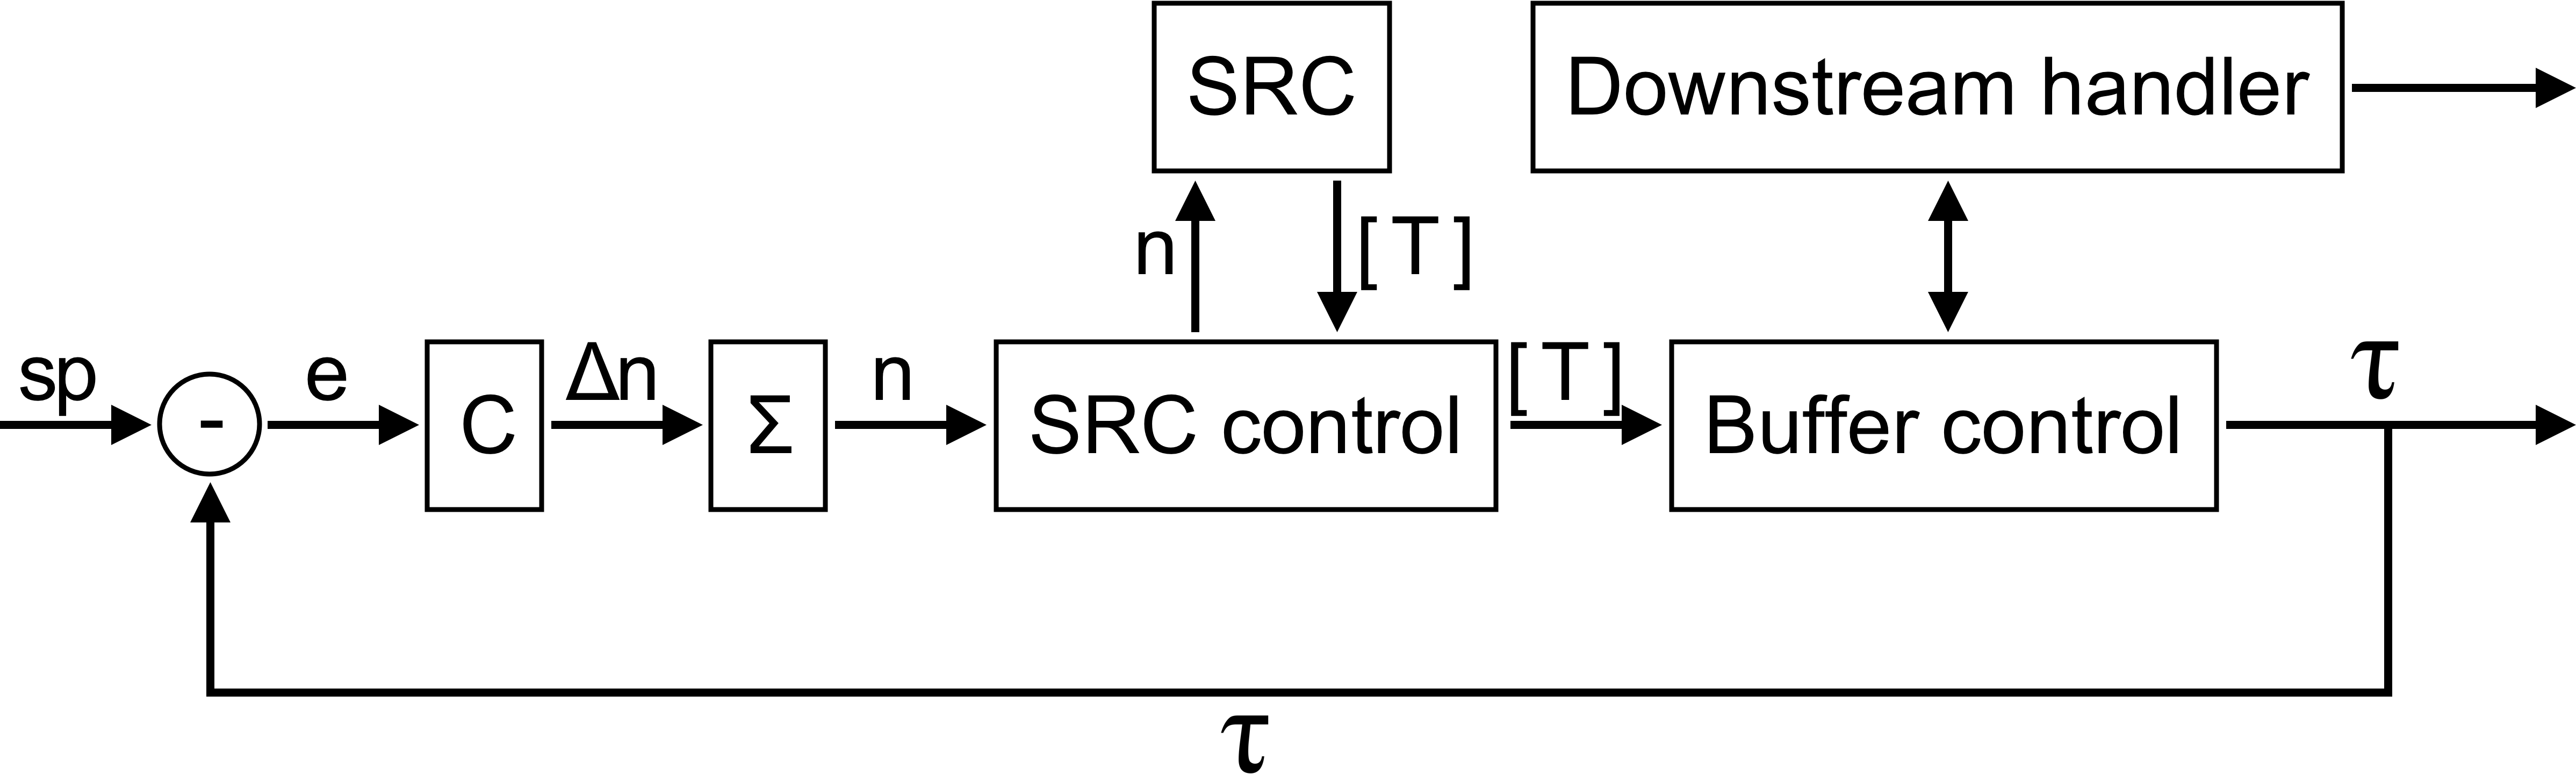
\includegraphics[width=0.8\textwidth]{figures/Backpressure-feedback-system.png}
	\end{center}
	\caption{Feedback system for controlling overproduction}
	\label{fig:backpressure-feedback-system}
\end{figure}

Compared to Reactive Streams and RxJava's reactive pull implementation, our approach has the major advantage of keeping the overflow protection to the only place it can be controlled from: the source of the stream. This allows us to keep the set of operators defined on the reactive interface clean and only have the responsibility of applying a specific functionality to the events that come in. Contrast this with RxJava's backpressure implementation where every operator has to also deal with the question of how many elements it is willing to receive next. This is equal to having our solution of controlling overproduction in every single operator.


\section{A universal, interactive interface}
As mentioned above, we propose to not wrap the (cold) source directly in \code{Observable.create}, but instead wrap it in a universal, interactive interface. This is necessary since there are many variants of interactive interfaces that all do the same, but each one in a slightly different way.

For example, the \itr interface has an \code{hasNext} and \code{next} method, which respectively check if there is a next element and return the next element. C\#'s \ier on the contrary has methods such as \code{moveNext}, which fetches the next element and returns whether there is a next element, and \code{current}, which actually returns the next element. For SQL database interaction, Java defines a \code{ResultSet}. This interface has a method called \code{next}, which moves the cursor to the next row of the result, and methods such as \code{getInt(int columnIndex)} and \code{getString(int columnIndex)} to get the content of a specific type from a column in the row the cursor is pointing to.

One thing these interfaces have in common is that they contain a method that fetches a single element and in the mean time block the thread it is operating on. If this fetch takes some time, your program will have to wait for the result to come in. To prevent this blocking behavior, we propose a universal interactive interface in which you request an element and subscribe to a stream on which \textit{eventually} this element will be emitted. Note that we separate the concerns of \textit{requesting} a next element and \textit{receiving} a next element. In this way, the program can still continue to operate and maybe do some other things while it is waiting for the requested element.

Given that we will use this interface in a feedback system that controls a buffer, we will pose an extra requirement on this interface. As the feedback system's controller might conclude that $n > 1$ elements need to be requested from the source, we must have to possibility to do so. Rather than $n$ times requesting 1 element, we want to request $n$ elements at once.

The complete interface is called \code{Requestable[T]} and is shown in \Cref{lst:universal-interactive-interface}. It contains a single abstract method \code{request(n: Int): Unit}, which is called whenever the user of this interface wants a certain number of elements from the source. The requested elements will at some point in time be emitted by the \obs that is returned by \code{results: Observable[T]}. If no more elements are available in the source, this \obs will terminate with an \code{onCompleted} event. The implementor of \code{Requestable} is expected to use the \code{subject} to bring elements in the stream, whereas the user of the interface is expected to observe \code{results} in order to get the requested data. Note that this is a \emph{hot} stream: element emission will not be repeated as a second \obv subscribes to the stream.

Example implementations of this interface for \itr and \code{ResultSet} are included in \Cref{app:backpressure-solution}.

\begin{minipage}{\linewidth}
\begin{lstlisting}[style=ScalaStyle, caption={Universal, interactive interface used in the feedback system}, label={lst:universal-interactive-interface}]
trait Requestable[T] {

  protected final val subject $=$ PublishSubject[T]()

  final def results: Observable[T] $=$ subject

  def request(n: Int): Unit
}
\end{lstlisting}
\end{minipage}


\section{Controlling overproduction using feedback control}
Now that we are able to interact with any cold source via the \code{Requestable} interface, we can continue designing and discussing the actual feedback system that controls the size of the bounded buffer. As stated before, we do not control the \emph{actual} size of the buffer by using a setpoint of any arbitrary, fixed number of elements. Instead we observe how many elements were taken out of the buffer in relation to how many elements were in the buffer during a particular time span. With that we do in fact not control the buffer's \emph{size}, but rather control the \emph{throughput} of the buffer, while making changes to the number of elements that are requested from the source at every feedback cycle.

The throughput in a particular time span ($\tau_t$) is defined in terms of how many elements are there to be consumed in relation to how many of these elements are actually being consumed. In a scenario where the elements that are not consumed in a certain time span are discarded or where the buffer is flushed at the end of each time span, the throughput would be equal to the ratio of how many elements were being consumed to how many elements were presented to be consumed in a certain time span. In our case, however, we do not wish to discard any elements but rather keep the left-over elements from the previous time span and make them part of what is available to be consumed in the next time span. With this we can define the throughput $\tau_t$ at time $t$ as

\begin{equation}\label{eq:throughput-fraction}
\tau_t = \frac{q_{t-1} + n_t - q_t }{q_{t-1} + n_t} \text{ \textbf{with} }q_{t-1}\text{, }q_t\text{, }n_t\text{ integers} \geq 0
\end{equation}

or

\begin{equation}\label{eq:throughput-simple}
\tau_t = 1 - \frac{q_t}{q_{t-1} + n_t} \text{ \textbf{with} }q_{t-1}\text{, }q_t\text{, }n_t\text{ integers} \geq 0
\end{equation}

In these formulas, $q_t$ is the size of the buffer at time $t$, whereas $n_t$ is the number of elements that has been put in the buffer between time $t - 1$ and $t$.

\Cref{eq:throughput-simple} provides us with a sense of the range of $\tau_t$. Since $q_t \leq q_{t-1} + n_t$ (it is not possible to take out more elements than are present in the buffer) we can guarantee a lower bound for $\tau_t$ of $0.0$. Likewise, since $q_{t-1}, q_t, n_t \geq 0$, we can set an upper bound for $\tau_t$ of $1.0$. Still there is the possibility of dividing by 0, but we will guard against this in the next couple of paragraphs.

\begin{equation}\label{eq:range-of-tau}
0.0 \leq \tau_t \leq 1.0
\end{equation}

With $\tau$ as the metric for the feedback system that controls the buffer, it is not difficult to come up with an appropriate setpoint. We want the throughput to be as high as possible, which is, given \Cref{eq:range-of-tau}, $1.0$.

The next point in designing this feedback loop is to determine when a new cycle starts. For this we have to observe that it will only make sense for a new cycle to start if the downstream has polled at least one element from the buffer. If in a certain time span the downstream is too busy processing one element, it does not make any sense to do a new measurement of the throughput. As new elements have been coming in based on the previous feedback cycle, but no elements have been taken out of the buffer, we do not need to request more elements. Instead, we just extend the time span by merging it with the next, until at least one element has been taken out of the buffer. Only then the feedback loop will run a new cycle.

Note that using this definition of a feedback cycle is a guard against dividing by 0 in \Cref{eq:throughput-fraction,eq:throughput-simple}. This can only happen when at the start of a time span the buffer is empty and during this time span no elements are coming into the buffer. This can either be due to an unfortunate decision of the controller (which we will discuss in \Cref{subsec:controller-design}) the request no further elements from the source, even though the buffer is empty, or because it takes some amount of time before the source can produce its next element. If the buffer was empty at the start and no elements were coming in, the downstream would at no point during this time span be able to poll an element from the buffer. Because of this, the current time span is merged with the next time span, without running through a whole new cycle and therefore also without running into dividing by 0 while calculating $\tau$.

\subsection*{Implementation}
With this metric and its constraints in mind, we can start implementing this system using the feedback API as described in \Cref{chap:feedback-api}. For now we will assume the existence of the controller that will be used in this feedback system, even though it will only be discussed first in \Cref{subsec:controller-design}. We assume a value \code{controller} of type \code{Component[Double, Int]}, with an input as the difference between the setpoint value and the actual throughput, and an output as the number of elements to be requested from the source. We furthermore assume the existence of a value \code{source} of type \code{Requestable[T]} from which we can request these element of a generic type \code{T}.

The buffer is modeled as a \code{BlockingQueue[T]}, such that multiple threads (to put and poll respectively) can safely interact with it. Besides that we introduce two flags of type \code{AtomicBoolean}, which signal respectively whether the source is completed (it has no more values) and whether there has been a successful poll during the current feedback cycle.

The code for the feedback system itself is shown in \Cref{lst:buffer-feedback-control}. Given the controller, we first send the number of requested elements to the source, which then starts producing at most this amount of elements. These are received by the feedback system by listening to \code{source.results}. These elements are then put into the queue.

To measure the throughput of the buffer, we collect the elements during a certain interval. From this we measure how many elements have come in the queue, as well as the total number of elements that are currently in the queue. As a side-effect we reset the flag for \code{pollerVisited} to false, since we are now done interacting with the queue. Also, we provide a default starting value for the feedback system at this point, since initially the queue was empty and no elements were going in the queue. It is necessary to do so, as we next compare the current situation with the previous situation by using a \code{buffer(2, 1)}. Finally, we compute the throughput as described in \Cref{eq:throughput-fraction}. This value is fed as the input of the next feedback cycle without performing any operations on the way back.

\hspace*{-\parindent}
\begin{minipage}{\linewidth}
\begin{lstlisting}[style=ScalaStyle, caption={Feedback system for controlling the buffer}, label={lst:buffer-feedback-control}]
controller
  .tee(n $\Rightarrow$ source.request(n))
  .liftRx(_.publish(_ $\Rightarrow$ source.results))
  .tee(x $\Rightarrow$ queue.put(x))
  .liftRx(_.buffer(interval.filter(_ $\Rightarrow$ pollerVisited.get()))) | \label{line:interval-in-feedback} |
  .map(in $\Rightarrow$ (in.size, queue.size))
  .tee(_ $\Rightarrow$ pollerVisited.compareAndSet(true, false))
  .startWith((0, 0)) // initially there is no input and the queue is empty
  .liftRx(_.buffer(2, 1))
  .filter(_.size $==$ 2)
  .map {
    case Seq((_, queueBefore), (in, queueAfter)) $\Rightarrow$
      (queueBefore - queueAfter + in).toDouble / (queueBefore + in)
  }
  .feedback(throughput $\Rightarrow$ throughput)
\end{lstlisting}
\end{minipage}

The rest of the code, the queue polling behavior, initialization of various values and the wrapping of the whole mechanic in an \code{Observable.apply}, are considered trivial. This can be found in \Cref{app:backpressure-solution}.


\section{A special controller}
\label{subsec:controller-design}
The final piece of this feedback control system is the controller, who's job it is to transform the difference between the setpoint and the throughput into a new number of elements to be requested from the source. However, before introduce the controller used in this control system, we first have to observe a number of issues.

We first have to consider the range of error values that is possible within this system. Since we have established that $\tau_t$ must be a value between 0.0 and 1.0 (\Cref{eq:range-of-tau}), and since we have set the setpoint to a value of 1.0, we must conclude that the range of values for the error must be between 0.0 and 1.0 as well (following \Cref{eq:tracking-error}). 

Although this bound may seem to be a good thing, it actually has some interesting implications on the controller of our choice. Janert observes in chapter 15 of his book \cite{janert2013-feedback} regarding this kind of bounds that they are not symmetric around the setpoint and that it is not even possible to have a negative error. For a standard PID controller to work well, it should preferably have a range of errors that is symmetric around the setpoint.

Janert suggests to solve this problem by not fixing the setpoint at 1.0 but put it ever so slightly below 1.0. With setpoints like 0.999 or 0.9995, he argues, we will do just as good, as the outcome of the controller will be an integer value rather than a floating point number. We are only able to add or subtract an entire element from the number to be requested. This however causes an unusual asymmetry in the tracking error. Although it can become negative, the error can become much more positive. Using a setpoint of 0.999, the tracking error on the negative side can be at most $0.999 - 1.0 = -0.001$. On the positive side, however, the tracking error can be at most 0.999, which is more than two orders of magnitude larger! As a control action originating from a PID controller is proportional to error, it becomes clear that control actions that tend to increase the number of requested elements will be more than two orders of magnitude stronger than control actions that tend to decrease the number of requested elements. Janert therefore concludes that this is not at all desirable and moves on to a completely new type of controller.

The problem that is discussed in chapter 15 of Janert's book is fairly similar to the situation at hand and so we will create a slightly modified version of his controller. We will keep the setpoint at 1.0, as stated in the previous section. Notice that with this the tracking error can never be negative. Also note that whenever $\tau_t = 1.0$, the tracking error will become zero. This can be interpreted as a signal from the downstream that it was completely able to keep up with the number of elements that were available in the buffer. Most likely this means that the number of requested elements was not high enough for the downstream to be kept busy all the time. We will therefore \textit{increment} the number of requested elements by 1 whenever this happens.

A tracking error greater than zero, on the other hand, signals that the downstream was not able to keep up with the total number of elements that were already present in the buffer and those that were added to the buffer in the previous cycle. We will take an optimistic approach here and assume that this is just an incidental occasion of less elements being consumed. Therefore we change nothing to the number of elements to be requested. We will however keep track of how many times in a row this situation of the tracking error being greater than zero occurs. Only if it happens a certain number of times in a row, we will \textit{decrement} the number of requested elements by 1. From that point on, we will monitor even closer and decrement once again (with briefer periods in between) if the throughput remains less than 1.0. If, however, the throughput comes back to 1.0, we consider it to be a satisfying number of elements, stop decrementing and slowly start increasing the number of requested elements again.

\subsection*{Implementation}
As the attentive reader may already have noticed, this is an incremental controller: it does not state how many elements should be requested next, but rather return by how many the number of elements to be requested should be increased or decreased. The actual number is calculated by an extra component added right after the controller, which does the integration over all historical $\Delta n$'s.

The controller itself is basically a stateful class with a transformation method to construct the next state. Furthermore we have an initial state defined on this class to get everything started. Using the API defined in the previous chapter, we can wrap this state into a \code{Component} using RxMobile's \code{Observable.scanLeft} operator. After the newest $\Delta n$ is extracted from this state, we use a \code{Component.scanLeft} to compute the actual $n$. In this step we also prevent the requested number of elements to go negative.

\begin{minipage}{\linewidth}
\begin{lstlisting}[style=ScalaStyle, caption={Controller implementation for controlling the buffer}, label={lst:buffer-controller}]
class Controller(time: Int, val change: Int) {
  def handle(error: Double): Controller $=$
    if (error $==$ 0.0) new Controller(period1, 1) // throughput was 1.0
    else if (time $==$ 1) new Controller(period2, -1)
    else new Controller(time - 1, 0)
}
object Controller {
  def initial $=$ new Controller(period1, 0)
}

val controller $=$ Component[Double, Controller](_.scanLeft(Controller.initial)(_ handle _))
  .drop(1)
  .map(_.change)
  .scanLeft(initialRequest)((sum, d) $\Rightarrow$ scala.math.max(0, sum + d))
\end{lstlisting}
\end{minipage}


\section{An API for cold sources}
With the development of a feedback system on buffer control as described in the previous sections, we can create an API that wraps an interactive source in an \obs, and let the feedback system draw elements from it based on how fast the downstream is able to handle these elements. To be more precise, given an interactive source, we can wrap it in a \code{Requestable} as described in \Cref{lst:universal-interactive-interface} and use the feedback system in \Cref{lst:buffer-feedback-control} to request elements from the source and put them in the buffer. Then the downstream mechanism will poll the buffer continuously and emit these elements in a reactive fashion to a sequence of operators followed by a final \obv. With this we can create a function called \code{from} that takes a \code{Requestable[T]} as its argument and returns an \code{Observable[T]} that emits all elements in the source.

\begin{minipage}{\linewidth}
\begin{lstlisting}[style=InlineScalaStyle]
def from[T](source: Requestable[T]): Observable[T]
\end{lstlisting}
\end{minipage}

The code for this function mainly consists of a combination of \Cref{lst:universal-interactive-interface,lst:buffer-feedback-control,lst:buffer-controller} and some glue to make it all work together. Refer to \Cref{app:backpressure-solution} for the full implementation.

One thing to highlight is that \code{from} not only takes the wrapped source as an input parameter, but also requires the interval at which the feedback system has to run. This is the \code{interval} which is used in \Cref{lst:buffer-feedback-control} \cref{line:interval-in-feedback} to determine when to do a next measurement of the throughput in the feedback system.

\begin{minipage}{\linewidth}
\begin{lstlisting}[style=InlineScalaStyle]
def from[T](source: Requestable[T], interval: Duration): Observable[T]
\end{lstlisting}
\end{minipage}

As one can imagine, this greatly influences the speed at which the elements are being emitted. If a source can emit elements immediately and the interval is set to 1 second, it will take much longer for all elements to be emitted than when it is set 1 millisecond. Of course the speed will ultimately be determined by how fast the downstream can consume any element. Given the discussion above on when a new feedback cycle is initiated by measuring the throughput, we can conclude that if \code{interval} is set too fast, it will not influence the performance of the system as a whole, as it will skip the intervals at which the downstream did not show any successful interaction with the queue. If, however, the interval is set at a slower rate than it takes for the downstream to drain the buffer, this will for obvious reasons negatively influence the performance of the system. One could propose to let \code{interval} be dynamically controlled using another feedback system. However, for now we decided to define it as a constant value in the system and make this part of future research.

With this we have created an API that creates an \obs from an interactive source while taking the possibility of overflow into account. Note that we did not have to change or add anything to the Rx interface. Instead we moved the overflow protection to the top of the operator chain, to the point where the source is polled directly. Now, when an \obv subscribes to the wrapped cold source, the feedback system will pull from the source on behalf of the \obv and push it as a reactive stream to the \obv.

To demonstrate the intended use of this API, we included a small example below in \Cref{lst:requestable-api-usage}. Here an iterable sequence is created, which is wrapped in a \code{Requestable.from}. We transform this into a regular \obs by calling the \code{observe} operator with an interval of \textit{1 millisecond}. This operator encapsulates the whole mechanic described in this chapter and will return the \obs that polls the buffer. Given this return value, we can now use all operators that are defined on \obs and complete the operator chain using a \code{subscribe}.

\hspace*{-\parindent}
\begin{minipage}{\linewidth}
\begin{lstlisting}[style=ScalaStyle, caption={Using the Requestable API to control the flow of a source}, label={lst:requestable-api-usage}]
val sequence: Range $=$ 0 until 133701
val slowConsumer $=$ Observer((i: Int) $\Rightarrow$ println("> " + i),
  e $\Rightarrow$ { e.printStackTrace(); System.exit(0) },
  () $\Rightarrow$ { println("done"); System.exit(0) })
		
Requestable.from(sequence)
  .observe(1 millisecond)
  .filter(_ % 2 $==$ 0)
  .map(2 *)
  .take(20)
  .subscribe(slowConsumer)
\end{lstlisting}
\end{minipage}

